\chapter{Signal Generating System}

\section{KAGRA Digital Control System}
The Digital Control System used in KAGRA is based on the Advanced LIGO Digital System \cite{dgs:overview}. In this system, analog control signals can be generated from a Digital-to-Analog Convertor(DAC) installed in any realtime computer known as a Front-End machine located around interferometer. Between the DAC output and experimental device, a customized analog low-pass filter called an Anti-Image filter \cite{dgs:aaai} has been installed for removing unwanted high frequency signal, the Image, due to digitized output from DAC. 

Inside a Front-End machine, the signal that will be sent to a DAC are prepared by a realtime software \cite{dgs:control.c}, which is generated from several building blocks, realtime models, by a customized parser and compiler \cite{dgs:rcg}. Each realtime model can be running at specifiable sample rate on a dedicated CPU core. However, currently, all DAC cards installed at KAGRA site are 16bit, 64kHz (65536Hz) ones. Therefore, a mandatary model named Input/Output Processor(IOP) model will always run at 64kHz \cite{dgs:control.c}, communicating with a DAC card and other "slave" models, in which people can put digital filters, signal generators, etc \cite{dgs:software_app}.



On the other hand, the digital system also works as a Data Acquisition System (DAQ). An analog signal coming from a transducer (e.g.~a photodiode) can be sampled by an Analog-to-Digital Convertor(ADC). After that, processed by optional digital filters, it could be sent back to an experimental device trough a DAC, be analyzed by an online diagnosis tool, or be stored into a frame file through the frame-builder. To avoid aliasing effect, which is caused by a finite sampling rate, a customized analog low-pass filter, which has the same circuit design as the AI filter, called an Anti-Alias filter \cite{dgs:aaai} has been inserted between the incoming signal and the ADC card.
%\red{ Reference!!! Reference!!!}

Unfortunately, the noise performance of such general purpose system do not meet the requirement of KAGRA Photon Calibrator in current setup. The noise coming from the digital system output can be directly translated into the PCal laser intensity noise, which will displace the ETM in a noisy way.   

\begin{figure}[hbt!]
\centering
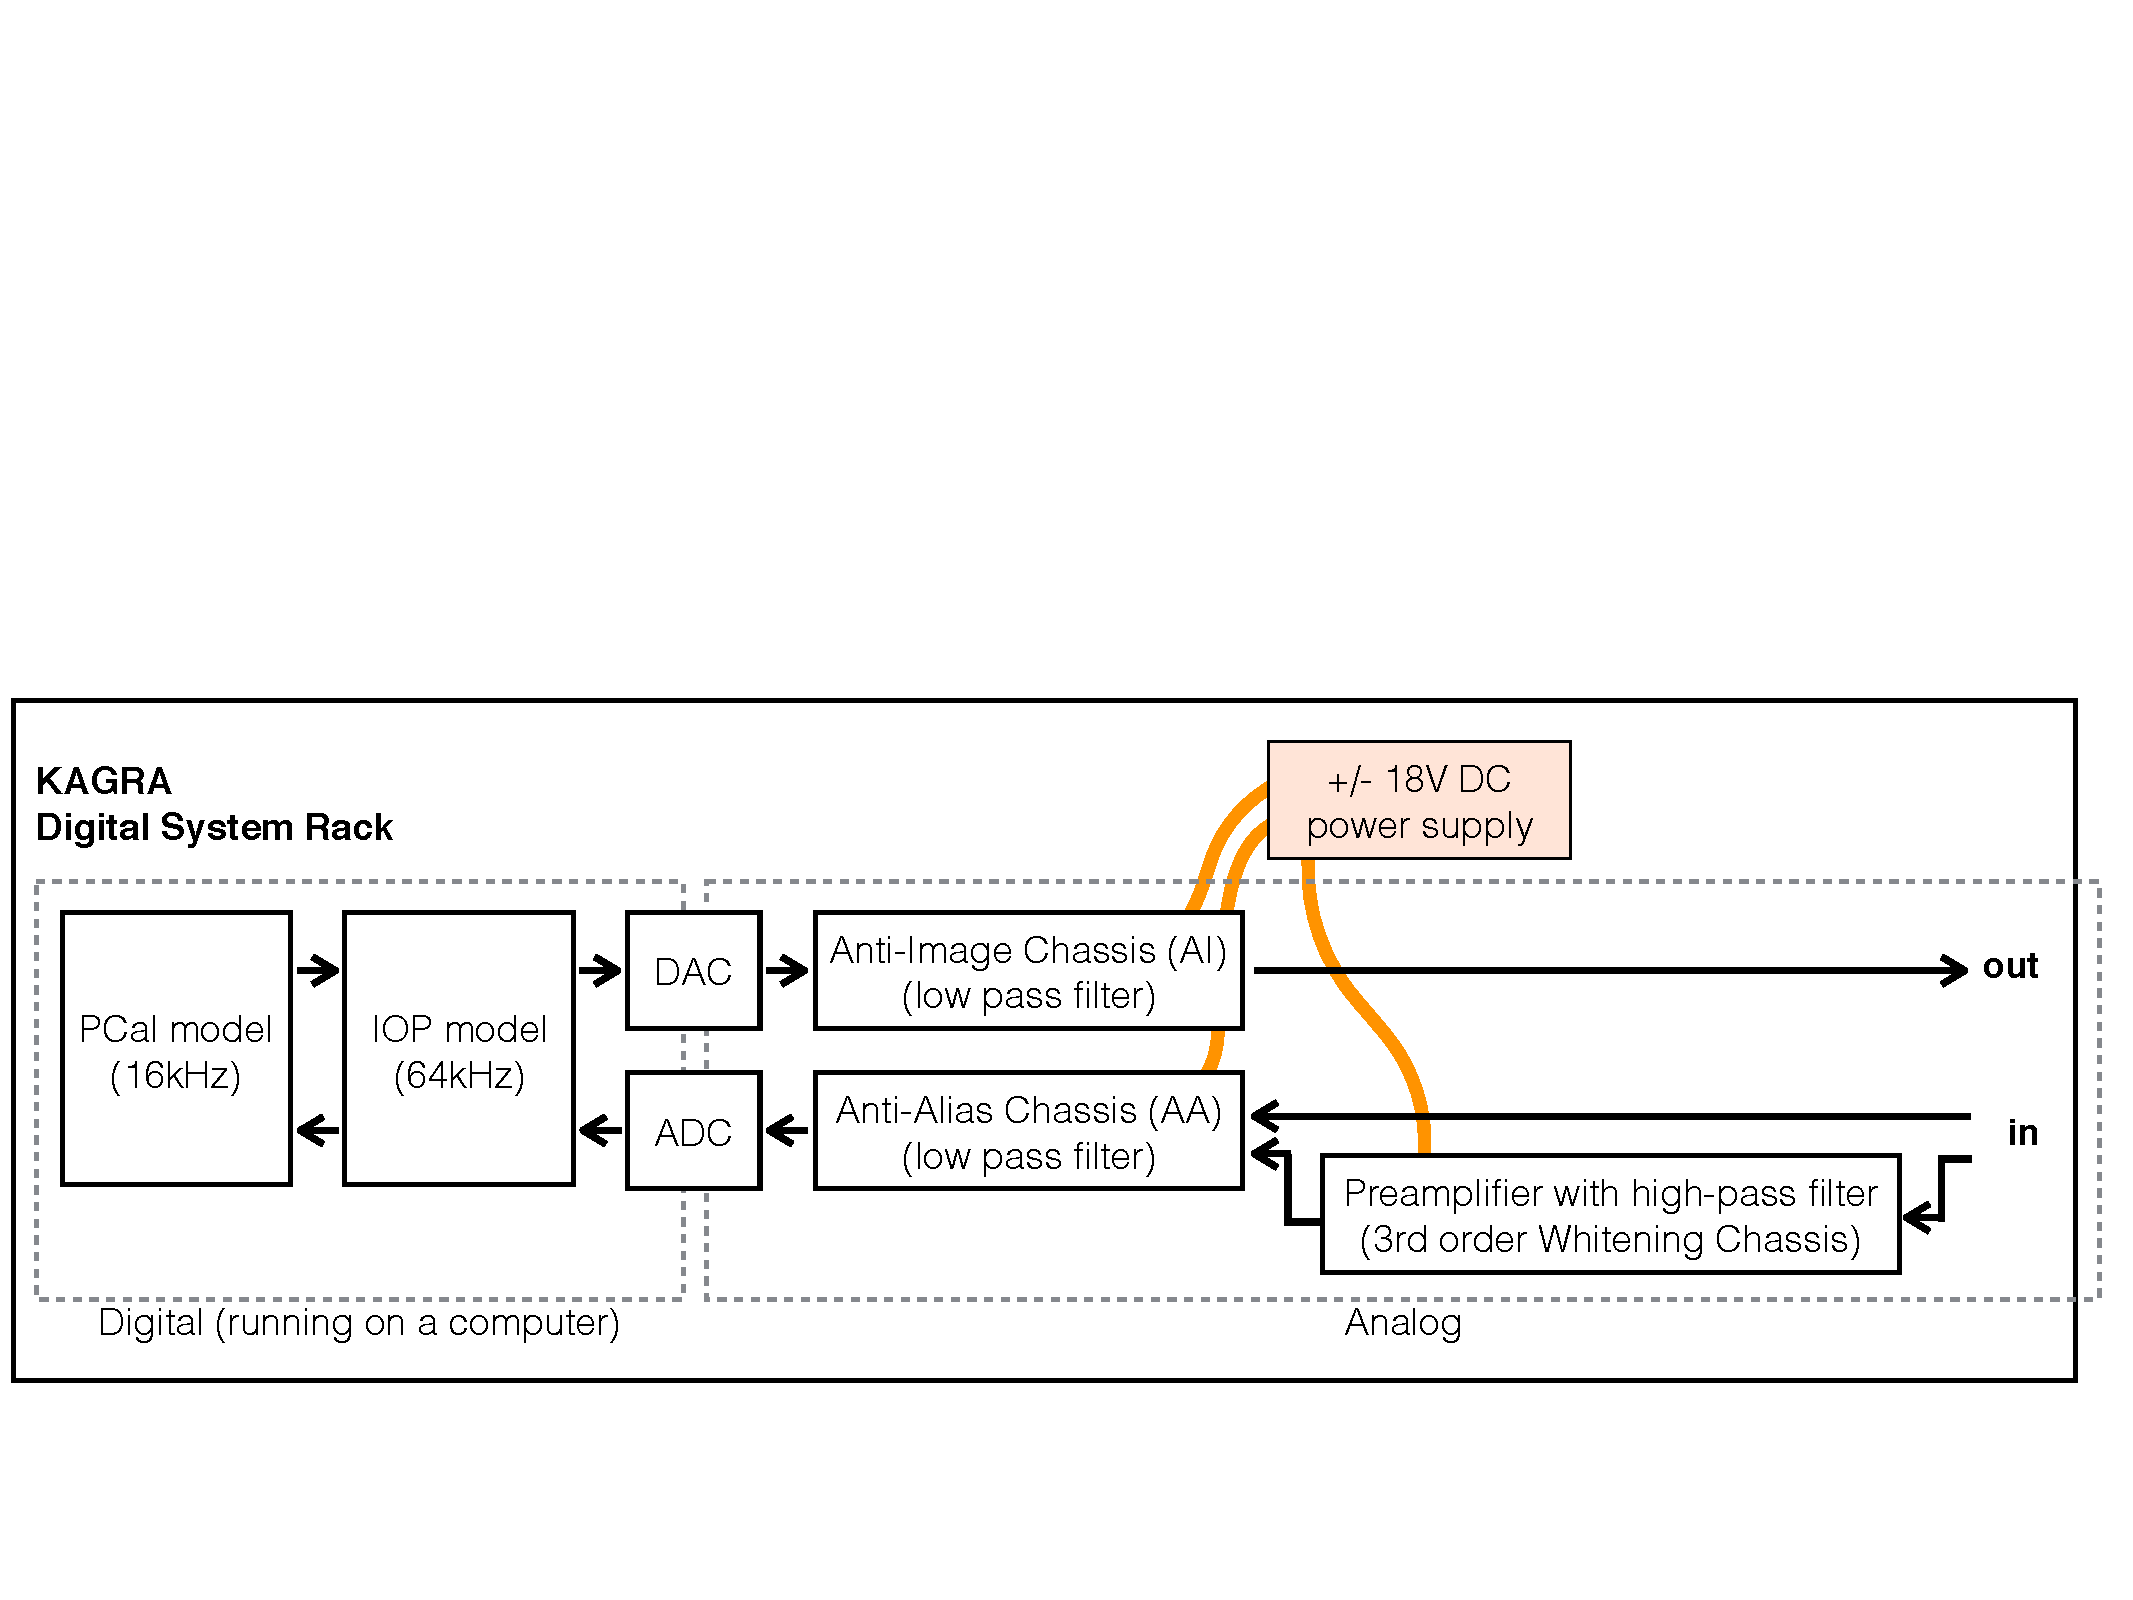
\includegraphics[width=1\textwidth]{figure/dgs_rack}
\caption[dgs]{The schematic shows the inside of the KAGRA digital system block in Fig.~(\ref{fig:injsigpath}). A optional whitening chassis is used as a preamplifier that only amplify the signal above 10Hz.     }
\label{fig:dgs_rack}
\index{figures}
\end{figure}


\begin{figure}[hbt!]
\centering
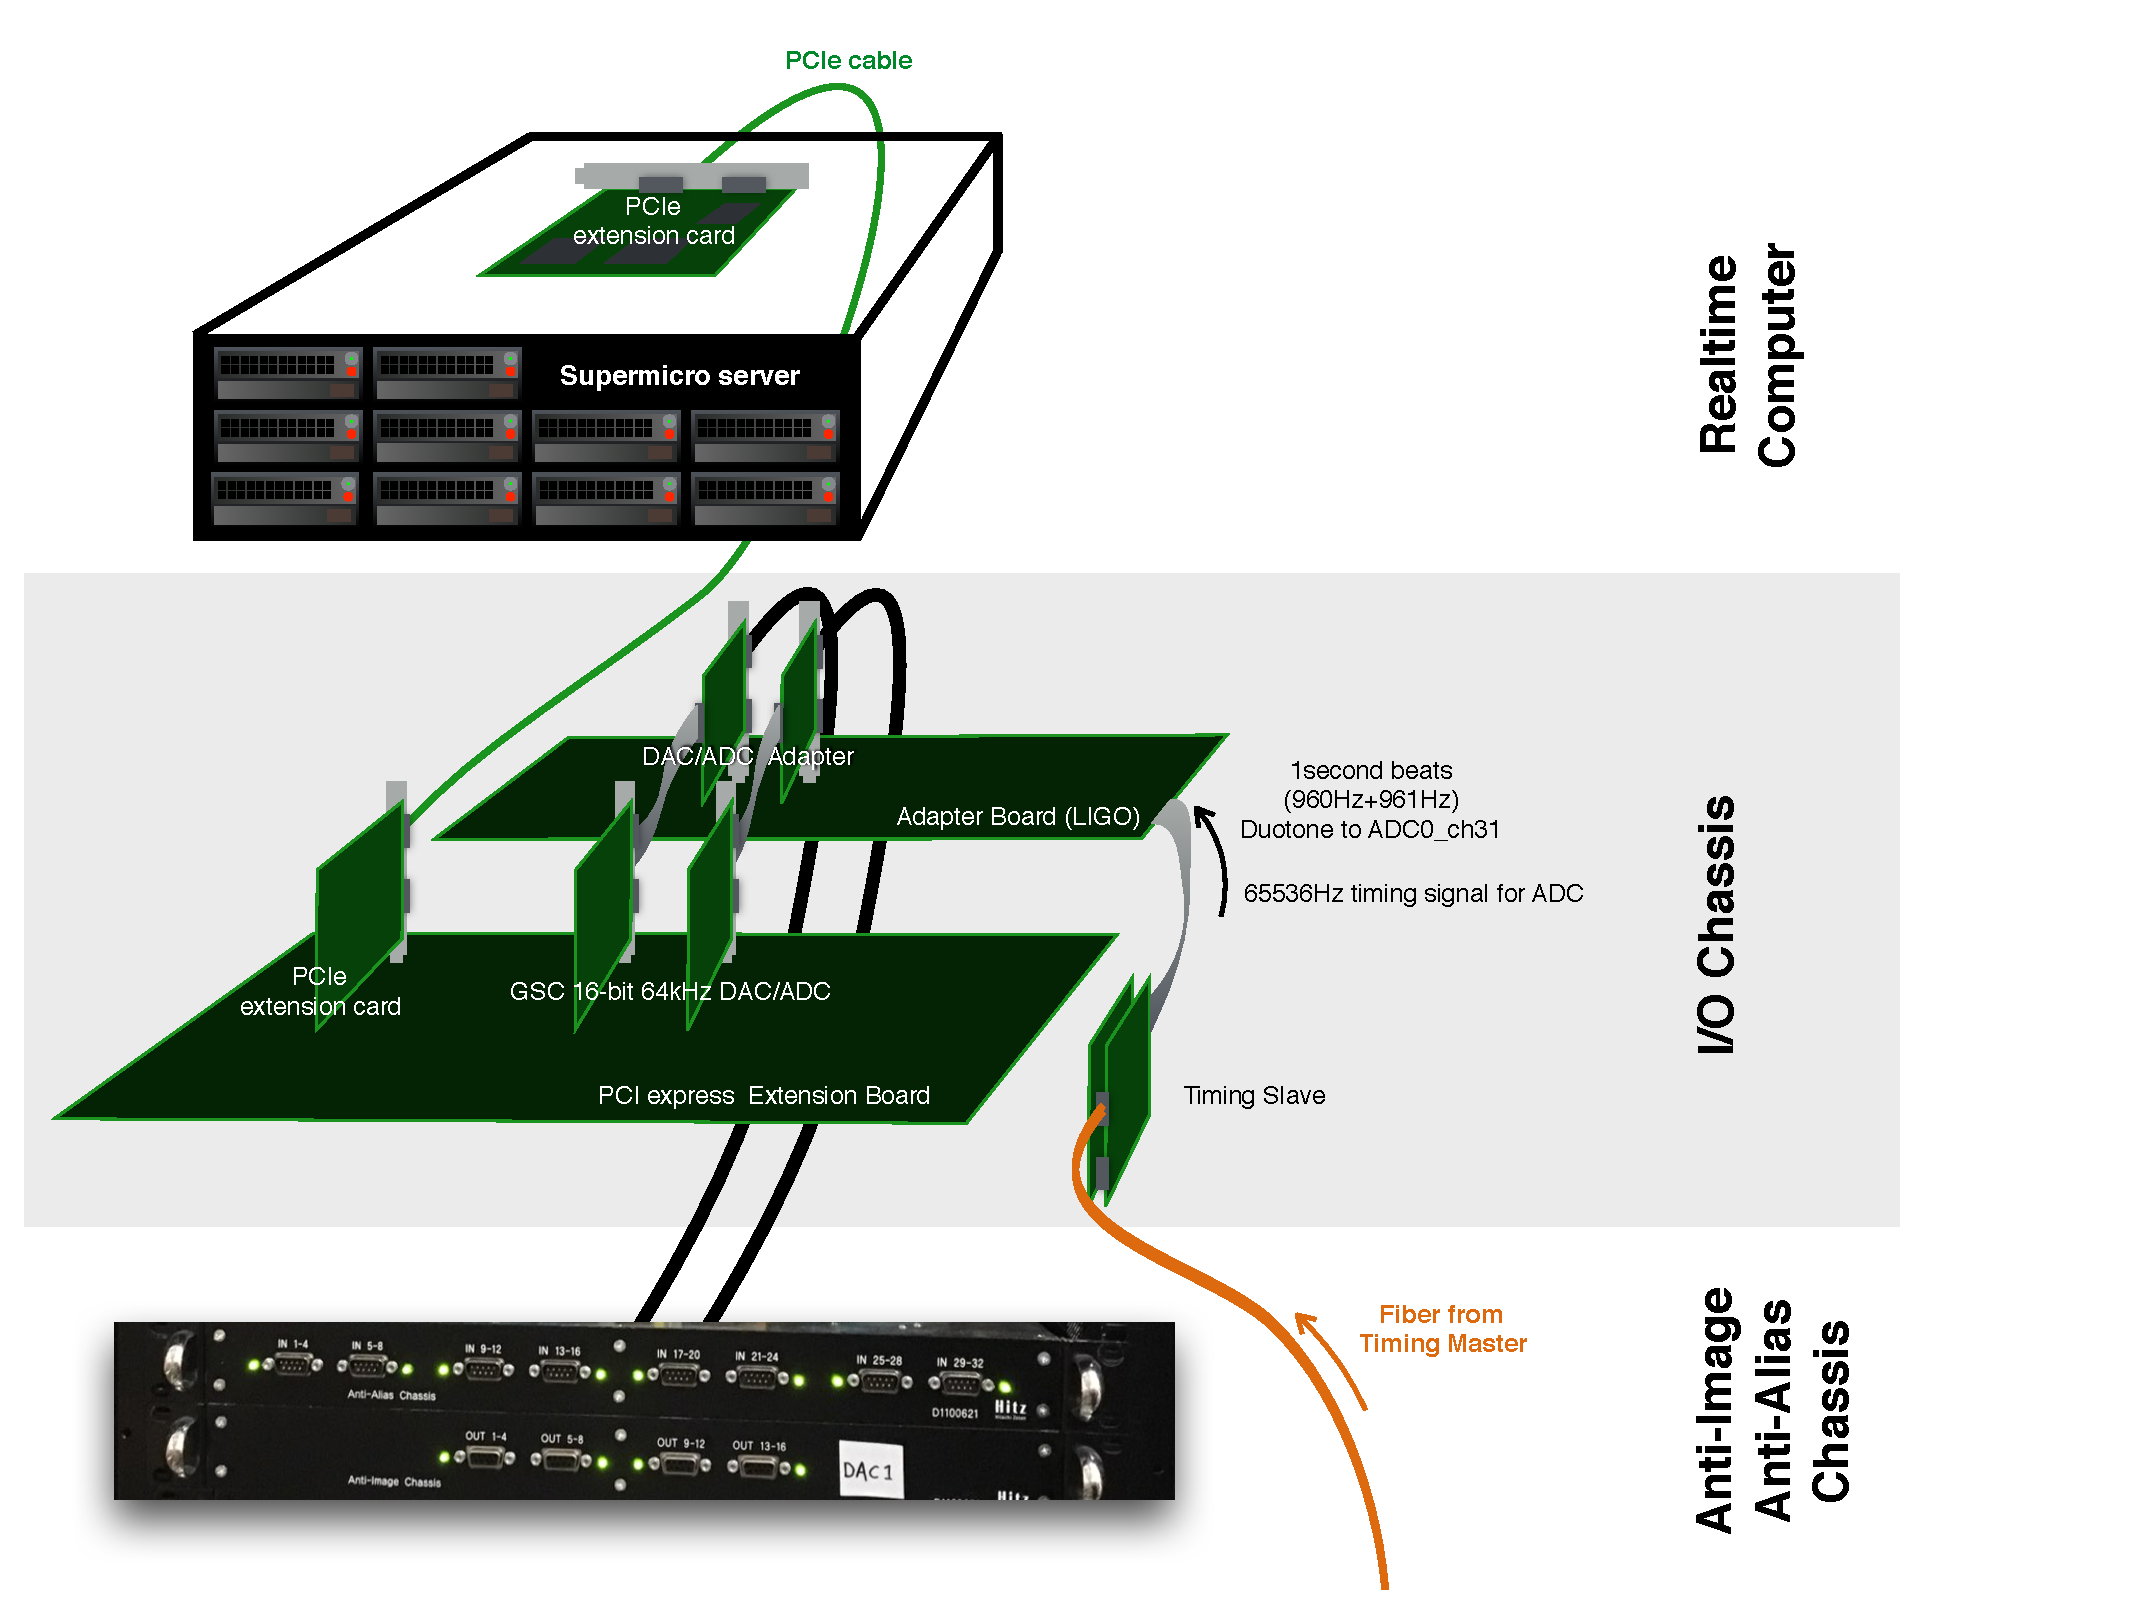
\includegraphics[width=1\textwidth]{figure/dgs}
\caption[An example schematic of a Digital System Rack]{ An example schematic of a Digital System Rack. As a user of Digital system, you may connect your experimental device to the D-sub 9 pin connectors in the front panel of AA/AI chassis. The conversing between analog and digital signal can be done by ADC and DAC cards inside the I/O chassis. In order to synchronize different ADC/DAC cards located over the whole interferometer, a Time Distribution System (TDS) has been build. It receive the timestamp from a GPS antenna and try to synchronize all Timing Slaves to a central Timing Master. Then, in all I/O chassis, synchronized timing slaves can generate clock signals simultaneously.  }
\label{fig:dgs}
\index{figures}
\end{figure}



\clearpage
\section{Noise Problem of Injection Signal}

The noise contains in the injection signal should not excess the sensitivity curve of the main interferometer. Practically, a $1/10$ safety factor has been considered, which means we set our noise requirement as ten times below the KAGRA sensitivity.  


\begin{figure}[hbt!]
\centering
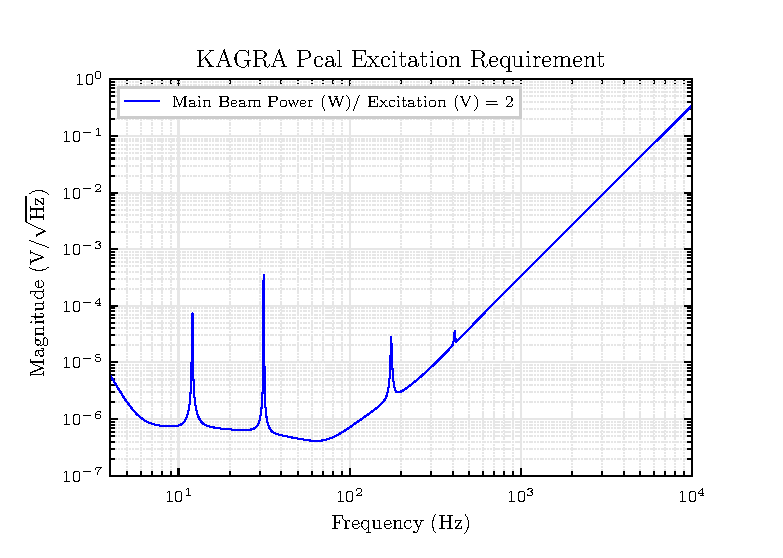
\includegraphics[width=.9\textwidth]{figure/DAC_requirement.eps}
\caption{Injection Channel Noise Requirement}\label{fig:DAC_noise_requirement}
\index{figures}
\end{figure}

\begin{align}
%\label{eq:}
   \Delta L(f) &< \frac{1}{10} \times (\text{KAGRA length sensitivity})\\
   \Delta L(f) =\frac{2 \Delta P(f) \cos(\theta)}{c} \frac{1}{M(2 \pi f)^2} &< \frac{1}{10} \Delta h(f) L
\end{align}




\subsection{Noise Sources from Control Signal}
\subsubsection{Quantization Noise of DAC}


The origin of quantization error is coming from the difference between desired analog output and quantized Digital to Analog Converter(DAC) output value. Roughly speaking, it shows up like white noise that is spread from DC to Nyquist frequency, i.e. $Fs/2$.
The Root Mean Square value of quantization noise has the order of voltage difference corresponding to last digit or Least Significant Bit(LSB). In time domain, we can calculate standard deviation.
\begin{align}
%\label{eq:}
   \sigma_x = \sqrt{\frac{1}{12}} \delta x_{LSB}
\end{align}

For a 16-bit 64kHz DAC with output range between $\pm 10$Volts, 
\begin{align}
%\label{eq:}
    \sigma_x &= \sqrt{\frac{1}{12}} \delta x_{LSB} \\
             &= \sqrt{\frac{1}{12}} \frac{(+10)-(-10) \mathrm{Volts}}{2^{16}} \\
             &= 8.81 \times 10^{-5} \;\mathrm{Volts}
\end{align}

In frequency Domain, the quantization noise is distributed from DC to 32768Hz; therefore, we have ASD
\begin{align}
%\label{eq:}
    ASD &= \sqrt{PSD} \\
        &= \sqrt{ \frac{\sigma_x^2}{32768} } \\
        &= 8.81 \times 10^{-5} \sqrt{\frac{1}{32768}} \\
        &= 4.87 \times 10^{-7} \;\mathrm{Volts}/\sqrt{\mathrm{Hz}} 
\end{align}

\subsubsection{Analog circuits}


\subsubsection{AC Power Line}


